\section{Part B - Analysis and Controller Design}%
\label{b}


Henceforth, a set of values are assumed to carry out simulations : $m = 0.425kg$, $g=9.81m/s^2$, $d = 0.42m$, $\delta = 0.65m$, $r = 0.125m$, $R = 53\omega$, $L_{0} = 120mH$, $L_{1} = 25mH$, $\alpha = 1.2m^-1$, $c = 6815_{A^2 \cdot s^2}^{g\cdot m^3}$, $ k = 1880N/m$, $b = 10.4Ns/m$, $\phi = 42^{\circ} \\ 

\textbf{B1} \\
\textbf{B2} \\ 
Applying Sympy's diff functions, a set of linearised functions were derived which confirms theoretical calculation: \\
$A = \frac{4 V c}{\left(L + R y\right)^{2}}$ \\
$B = -\frac{2 k}{m}$ \\
$C =- \frac{2 b}{m}$ \\
Used in : \\
$\dot \bar x_{2} = A \bar V - B\bar x_{1} - C\bar x_{2} \\


\textbf{B3} \\ 
Determining impulse and step responses of the system of the transfer function \\
$$\frac{\bar x_{1}}{\bar V} = \frac{A}{S^2 + CS + B}$ \\$


\begin{figure}[H]
	\centering
	\captionsetup{justification=centering}
	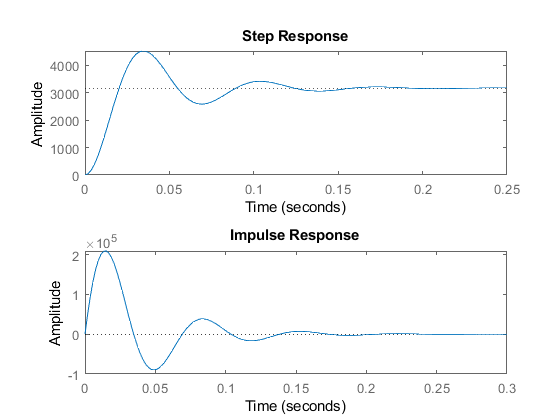
\includegraphics[width=1\linewidth]{imgs/Impulse step response.png}
	\caption{Amplitude responses over time of responses}%
	\label{fig:14}
\end{figure}

\textbf{B4} \\ 

\begin{figure}[H]
	\centering
	\captionsetup{justification=centering}
	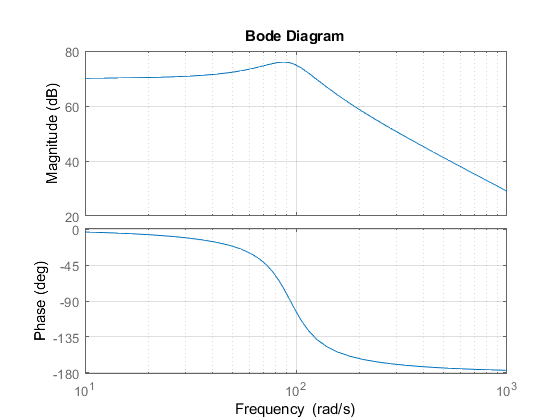
\includegraphics[width=1\linewidth]{imgs/Bode plot.png}
	\caption{Phase and Magnitude response over frequency sweep.}%
	\label{fig:14}
\end{figure}

\textbf{B5} \\ 